\chapter{Theoretical Foundations of Monotop Analysis}
\label{chapter:four}
This Chapter will focus on the explaining the theory behind the monotop analysis and the importance of the top quark.
\section{Monotop Analysis}

Great thoughts that further your argument. This includes lots of strong evidence presented throughout several paragraphs, each accompanied by necessary citations.
\begin{quotation}
    \noindent Here is a block quotation---a passage from a text you found insightful and wanted to share with others. Maybe it is from a journal article, website, or book. Irrespective, it should support the argument being made.\footnote{A citation for the quoted material.}
\end{quotation}
%Maybe a sentence or two that bring the argument and evidence together.\citep{dos_santos_2020}



\section{The Top quark}

The top quark was discovered at the Fermilab Tevatron almost 25 years ago. It is the weak isospin partner of the bottom quark. Its discovery resulted in completion of the three generation structure of the standard model (SM). The top quark mass was measured to be $m_{t} = 176 \pm 13$ GeV, a charge of 2/3 times the charge on the electron and a lifetime of $5 \times 10^{-25} s$ making it the heaviest of all the fermions known till date in the standard model. Because of it's large mass and correspondingly short lifetime it behaves differently than other quarks. 

The top quark decays before it hadronizes, passing its information to the decay products. Therefore making it possible to infer its properties from the decay products in the detector. The top quark decays into a a bottom quark and a W boson, and since the W boson is an unstable particle it decays into a quark anti-quark pair of different flavors (hadronic decay channel) or to a charged lepton and a neutrino (leptonic decay channel) with the following branching ratios.

\begin{table}[h!]
  \centering
  \caption{}
  \label{tab:average_channels}
  \begin{tabular}{cc}
    \toprule
     Decay channel &  Branching ratio \\
     \midrule
      $W^{\pm} \rightarrow q\Bar{q'}$ &   $68.32\%$  \\
      $W^{\pm} \rightarrow e^{\pm} \Bar{\nu_{e}}$ &   $10.46\%$  \\
      $W^{\pm} \rightarrow \mu^{\pm} \Bar{\nu_{\mu}}$ &   $10.50\%$  \\
      $W^{\pm} \rightarrow \tau^{\pm} \Bar{\nu_{\tau}}$ &   $10.75\%$  \\
      \bottomrule
  \end{tabular}
\end{table}

As the top quark decays into a W boson and a bottom quark, it's evident that the hadronic and leptonic decay probabilities of the top quark will be proportional to the hadronic and leptonic decay probabilities of the W boson. So, it can be implied from the above table that, around 70\% of times the top quark decays into three quarks (two quarks from W boson and one bottom quark) which further hadronize to produce jets. While around 30\% of the times the top quark would decay leptonically to a lepton, its corresponding lepton neutrino and a bottom quark. In this thesis we will be exploring the leptonic channel for the search for Dark Matter (DM), so our final state signature would a lepton, its corresponding neutrino and a jet coming from a bottom quark.

In accordance with the SM, at the LHC, top quarks are predominantly produced in pairs ($t \Bar{t}$) through strong interactions and as single top via the electroweak interaction. In the following section we will be looking at the production of a single top quark (Monotop) in association with missing transverse energy due to the two DM candidates, as an extension to the SM. 


\begin{figure} [tpb]
\centering
         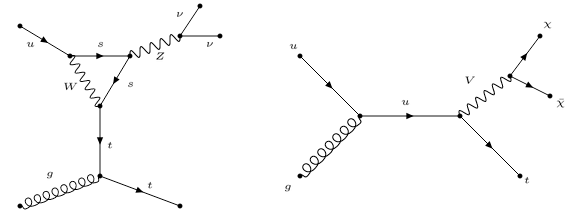
\includegraphics[width=0.9\textwidth,clip=]{thesis_template_cua/Figures/Feynman/tree_lebeL.png}
         \vspace*{10mm}
         \caption[Tree-Level Feynman]{ [Left]: Shows the tree-level Feynman diagram for Standard model monotop production. [Right] Shows the Leading-order Feynman diagram for the production of monotop signatures in the Dark Matter model \cite{monotoptheory:1}. It is flavor changing neutral interaction mediated by a hypothetical vector boson V decaying into two Dark Matter candidates $\chi$. }
         \label{theory:tree_level}
\end{figure}

\section{The Monotop Model}
This section details the theoretical motivation behind the monotop model \cite{monotoptheory:1}. The monotop model is based on an alternative approach  where a final state signature is proposed that no standard model process can reach at tree-level. The final state signature in our case is a top quark produced in association with missing transverse energy. In SM this production mode is suppressed both by a loop factor and by two powers of non-diagonal Cabibbo-Kobayashi-Maskawa matrix elements \cite{pham2011ckm:ckm}. In Figure \ref{theory:tree_level} we see that the left image shows the Standard model production of the monotop signature. The loop consisting of the W boson and two strange quarks allows for the production of Z boson and the top quark and if the Z boson decays into two neutrinos we get the monotop signature in accordance with rules of the Standard model. While the right image in Figure \ref{theory:tree_level} shows the tree-level production of the monotop signature. To allow for this tree-level production the monotop model suggests two main mechanisms \citep{monotoptheory:1}. Either the top quark is produced (resonantly or not) in association with missing energy of a fermionic nature or through a flavor-changing interaction with an invisible bosonic state, as illustrated on the left and right panels of Fig. \ref{theory:resonant}, respectively. This physics analysis utilizes the non-resonant monotop model so, we will discuss in detail about the flavor changing neutral interaction model (Non-Resonant model).

\begin{figure} [tpb]
\centering
         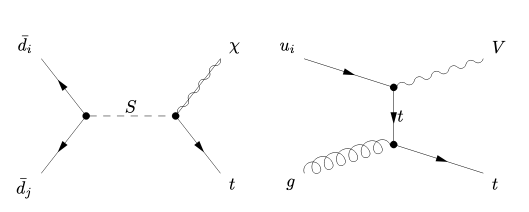
\includegraphics[width=0.9\textwidth,clip=]{thesis_template_cua/Figures/Feynman/res_non_res.png}
         \vspace*{10mm}
         \caption[Tree-Level Feynman Resonant]{[Left] Representative Feynman diagrams leading to monotop signatures, through the resonant exchange of a colored
         scalar field S and [Right] via a flavor-changing interaction with a vector field V (right). In these two examples, the missing energy is carried by the V and $\chi$ particles. The images have been adapted from \cite{monotoptheory:1}}
         \label{theory:resonant}
\end{figure}


\subsection{Non-Resonant Monotop Model}
As shown in the right panel of figure \ref{theory:resonant}, we see that a top quark is produced in association with an invisible bosonic field V (Spin 1). The invisible bosonic field couples with the top and light u/c quarks in a flavor changing way. There are two bosonic states associated with this non-resonant model, a bosonic vector field V with spin 1 and a bosonic scalar field with spin 0. These bosonic states are unstable because of their coupling to quarks. Since we are looking for a missing energy signature in the detector there are two ways in which that can be achieved in the monotop model. First, either the bosonic fields (Spin 0/Spin 1) are long lived such that, they decay outside the detector or, they decay into a pair of neutral stable particles. The monotop model discussed in this thesis would focus on the bosonic state decaying into two stable dark matter candidates. To ensure that the new invisible boson leads to missing energy signature in the detector, leads us to an assumption that bosonic field (V/$\Phi$) decays into dark matter candidates ($\chi, \Bar{\chi}$). The Lagrangian \cite{monotoptheory:2} for this (Flavor changing type interaction) model is 

\begingroup
\large
\begin{equation}
\mathcal{L} = \mathcal{L}_{SM} + \mathcal{L}_{kin} + 
\Phi\Bar{u}[a^{0}_{FC} + b^{0}_{FC}\gamma_{5}]u + V_{\mu}\Bar{u}\gamma^{\mu}[a^{1}_{FC} + b^{1}_{FC}\gamma_{5}]u + h.c.
  %\eta = -\ln\tan\left(\frac{\theta}{2}\right)
  \label{eq:lagrangian_monotop}
\end{equation}
\endgroup

$\mathcal{L}_{SM}$ is the Standard Model Lagrangian, which is supplemented by kinetic and gauge interaction terms for all new states included in the Lagrangian $\mathcal{L}_{kin}$. The third and the fourth terms describe the flavor changing associated production of the top quark and the invisible scalar $\Phi$ or a vector V, respectively. $u$ represents the up-type quarks (u,c,t) and the strength of the interactions of the two bosonic states (V/$\Phi$) and a pair of up-type quarks is modeled via two 3 $\times$ 3 matrices in flavor space $a_{FC}^{\{0,1\}}$ and $b_{FC}^{\{0,1\}}$. The monotop model is also chosen such that flavor changing neutral interaction only relates the up-type quark of the first generation with third generation of quarks. Which implies that all other coupling other than those between the first and third generation of quarks would tend to 0. i.e. $a_{1,3 (FC)}^{0,1}$ , $a_{3,1 (FC)}^{0,1}$ $\neq$ 0 and $b_{1,3 (FC)}^{0,1}$ , $b_{3,1 (FC)}^{0,1}$ $\neq$ 0, while all other couplings will have zero strength.

So, the main signatures associated with the monotop production can be classified according to the top quark decays.

$p p \rightarrow $$t + \cancel{\it{E}}_{T} \rightarrow b W + \cancel{\it{E}}_{T} \rightarrow b l \Bar{\nu_{l}} + \cancel{\it{E}}_{T}$ (Leptonic decay mode)

$p p \rightarrow $$t + \cancel{\it{E}}_{T} \rightarrow b W + \cancel{\it{E}}_{T} \rightarrow b j j + \cancel{\it{E}}_{T}$ (Hadronic decay mode)

In this thesis we will be using the leptonic channel for the search of dark matter candidates. Next section will include a detailed discussion about the vector and scalar invisible bosons.

\subsection{Spin 0 mediator}




\subsection{Spin 1 mediator}


\subsection{b-tagging and Deep Jet}


\section{Statistical Analysis Procedure}

\subsection{Fundamental Concepts}

Statistics plays a key role in particle physics. The CMS experiment collects data and this data is used either to make an inference about the probabilistic model (searching for a new phenomena) or to estimate the parameters of the model (precise measurements of a parameter of the SM, ex: the mass of the top quark). Such a statistical inference uses two main methods, first, the frequentist method which estimates the probability of an outcome by measuring the frequency of the outcome in a repeatable experiment. However one thing to note is that the frequentist method does not give the probability for a hypothesis or for the value of the parameter. The probability P(X) of an outcome X is defined as 

\begin{equation}
P(X) = \frac{\#\; of\; favorable\; outcomes}{\# \;of\; total\; possible\; outcomes}
  %\eta = -\ln\tan\left(\frac{\theta}{2}\right)
  \label{eq:frequentist}
\end{equation}

Second, the bayesian inference, it expresses one's degree of belief, for instance given a probability distribution function for a parameter, $f(x;\theta)$ we can express our degree of belief about the possible value that parameter can have. Bayesian inference is more like a subjective probability, it requires prior knowledge about the values that the parameter possesses before the experiment. With the usage of Bayes' theorem one can estimate the posterior probability of the parameter having a particular value.

\begin{equation}
P(Y|X) = \frac{P(X|Y)\; P(Y)}{P(X)}
  %\eta = -\ln\tan\left(\frac{\theta}{2}\right)
  \label{eq:Bayesian}
\end{equation}

In Eq \ref{eq:Bayesian},$P(Y|X)$ represents the probability of occurrence of Y under the assumption that X has happened and vice versa for $P(X|Y)$, $P(X)$ and $P(Y)$ are
called priors and represent the general probabilities for the outcome X and Y

